%*********************************************************************
%	CLOSED LOOP THERMAL PERFORMANCE
%*********************************************************************
\chapter{Closed Loop Thermal Performance}
\label{ch:ClosedLoop}


Chapter~\ref{ch:thermalID} identified both thermal plants from the built chamber. This chapter adds controllers to them and measures how the closed loops perform. Four tests were run, each building on the one before: how well the air temperature is held, whether hotter air warms the sample, whether heating from below does, and how evenly the heat reaches the plate.

%**********************************************************
\section{Controller Tuning}
\label{sec:cl-tuning}
%**********************************************************

Both controllers were tuned in Section~\ref{sec:sysid-gains}. The chamber uses $K_\mathrm{eff} = 32.6$ with $\tau = 775$\,s and $\lambda = 300$\,s, and the glass its own $K_{22} = 38.7$ with $\tau = 348$\,s and $\lambda = 60$\,s. In percent duty that gives $K_p = 7.90$ and $K_i = 1.02\times10^{-2}$ for the chamber, and $K_p = 14.99$ and $K_i = 4.31\times10^{-2}$ for the glass. The glass was tuned with $\tau = 348$\,s, the estimate available when the controller was written. Chapter~\ref{ch:thermalID} later settled on $370 \pm 25$\,s, which includes 348. The difference changes $K_p$ by 6\,\%, and Section~\ref{sec:cl-test2} shows no visible effect on the response, so the gains were left alone.

%*********************************************************************
\section{Implementation and Test Conditions}
\label{sec:cl-implementation}
%*********************************************************************


%*********************************************************************
Both loops run on the STM32 at $T_s = 1$\,s, in the same task that reads the sensors. The structure is the one designed in Section~\ref{sec:control-design}: PI with setpoint weighting $b = 0.5$ on the proportional term, clamping anti-windup, and duty limited to 0 to 100\,\%. The integrators are preloaded from the measured room temperature at start-up, so the loops begin at a sensible duty. Duty reaches the heaters by time proportioning on the PWM channels, and an over-temperature trip cuts both heaters if any channel exceeds the limit set for the run.

Every run logs all channels at 1\,Hz, along with both duties and the condensation margin. The margin is the glass temperature minus the chamber air temperature, and it must stay positive to keep the optical path clear. Sensor placement follows Section~\ref{sec:sysid-approach}, and Table~\ref{tab:cl-conditions} lists what changed for each test. No faults, trips or sensor-loss events occurred in any of the four runs.

%*********************************************************************

\begin{table}[htbp]
    \centering
    \caption{Conditions for the four closed loop runs.}
    \label{tab:cl-conditions}
    \small
    \begin{tabular}{llllll}
        \toprule
        \textbf{Run} & \textbf{Length} & \textbf{Setpoints} & \textbf{Plate lid} & \textbf{Base Heat} & \textbf{Well probes} \\
        \midrule
        1 & 3\,h 23\,min & 37 / 39\,\textdegree{}C & on   & none    & one well, mid depth \\
        2 & 3\,h 19\,min & 39 then 43 / 48\,\textdegree{}C & off & none & centre and edge, at the bottom \\
        3 & 3\,h 12\,min & 39 / 48\,\textdegree{}C & off & 0, 20, 45\,\% & one well, at the bottom \\
        4 & 3\,h 54\,min & 39 / 48\,\textdegree{}C & off & 45 then 30\,\% & wells E8 and H12 \\
        \bottomrule
    \end{tabular}
\end{table}

%*********************************************************************
\section{Holding the Setpoint}
\label{sec:cl-test1}
%*********************************************************************

The first run tests three things: how well the air holds 37\,\textdegree{}C, whether the sample follows it, and how the loop recovers from a disturbance. The plate had its lid on and water in the wells, the glass setpoint was 39\,\textdegree{}C, and the chamber was opened by hand at $t = 11\,110$\,s. Figure~\ref{fig:C1-regulation} shows the run.

\begin{figure}[htbp]
    \centering
    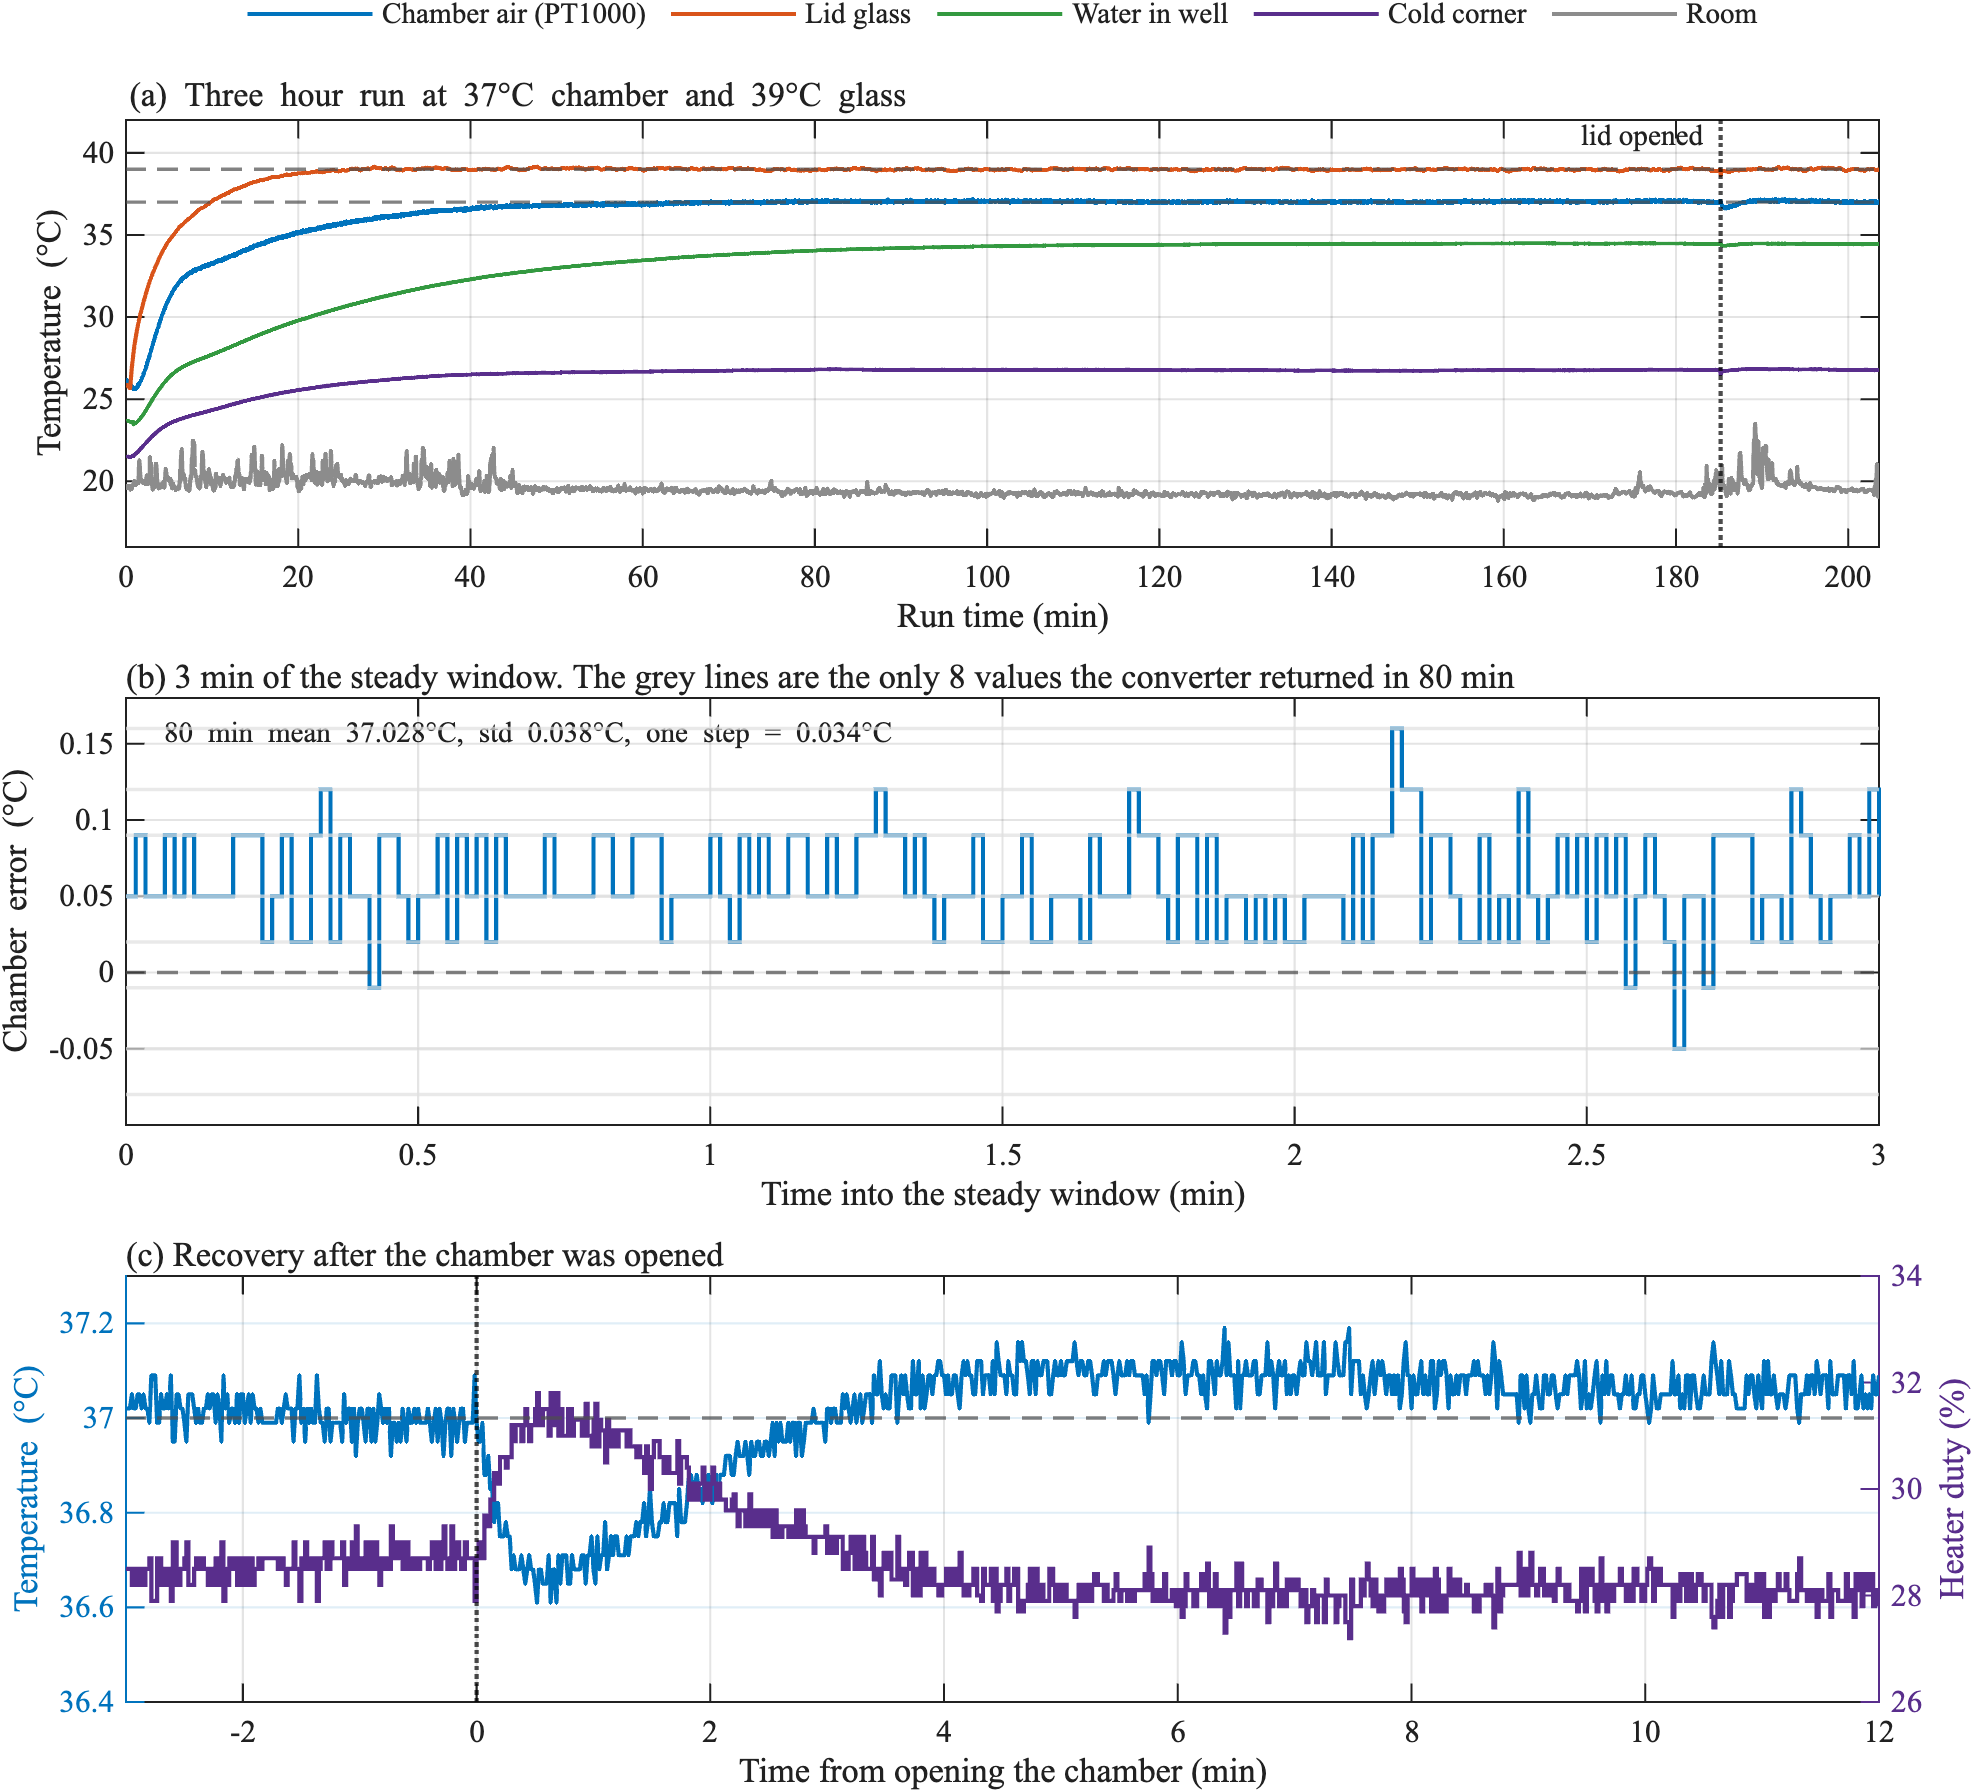
\includegraphics[width=0.66\textwidth]{figs/ch7/fig_C1_regulation.png}
    \caption[Regulation at 37 and 39 degrees]{\textbf{Holding 37\,\textdegree{}C chamber and 39\,\textdegree{}C glass for three hours.} (a) The whole run, with the moment the chamber was opened marked. (b) A 3 minute slice of the steady window; the grey lines are the only values the converter can return, so the regulation is at the measurement floor. (c) Recovery after the chamber was opened, with the heater duty on the right axis.}
    \label{fig:C1-regulation}
\end{figure}

\textbf{Warm-up.} On a 60\,s moving average the chamber reached $\pm$1.0\,\textdegree{}C in 28.4\,min, $\pm$0.5\,\textdegree{}C in 36.9\,min and $\pm$0.2\,\textdegree{}C in 48.8\,min. The glass reached the same bands in 13.3, 16.5 and 20.7\,min, about 2.3 times faster. The glass settles while the chamber is still about 2\,\textdegree{}C short, so for most of the warm-up and all of the steady run the chamber loop sees a fixed glass temperature. That is what the decoupled design needs.


Neither loop overshot. The chamber rose to 37\,\textdegree{}C and held within the measurement resolution, and the glass reached 39\,\textdegree{}C at about 30 minutes and did not go past it. That is what the setpoint weighting of $b = 0.5$ was introduced for in Section~\ref{sec:control-design}, where a standard PI overshot by 0.48\,\textdegree{}C in simulation. Neither loop saturated at any point in this run.

\textbf{Steady state.} Table~\ref{tab:cl-test1-steady} gives the averages over the 80 minutes before the chamber was opened.

\begin{table}[htbp]
    \centering
    \caption{Steady state over 80 minutes, run 1.}
    \label{tab:cl-test1-steady}
    \small
    \begin{tabular}{lccccccc}
        \toprule
         & \textbf{Chamber} & \textbf{Glass} & \textbf{Well} & \textbf{Corner} & \textbf{Room} & \textbf{Wall duty} & \textbf{Glass duty} \\
        \midrule
        Mean    & 37.028 & 38.987 & 34.438 & 26.767 & 19.204 & 29.2\,\% & 26.3\,\% \\
        Std dev & 0.038  & 0.040  & 0.047  & 0.020  & 0.130  & 0.45     & 1.03 \\
        \bottomrule
    \end{tabular}
\end{table}

The sensor sets the limit here, not the controller. One MAX31865 step is 0.034\,\textdegree{}C on a PT1000, and across the whole 80 minutes the chamber channel returned only eight distinct values, spanning 0.24\,\textdegree{}C. The standard deviation of 0.038\,\textdegree{}C is the spread of those eight levels. Nothing tighter than $\pm$0.04\,\textdegree{}C can be claimed with this instrumentation, and nothing tighter is needed. The fairer comparison with R1 is the full span: every reading in the 80 minutes lay within 0.24\,\textdegree{}C, or about $\pm$0.12\,\textdegree{}C, which uses less than half of the $\pm$0.3\,\textdegree{}C that R1 allows. The numbers above say how little the chamber moved, not how close 37.028\,\textdegree{}C is to a true 37\,\textdegree{}C. That depends on the calibration in Section~\ref{subsec:pt1000-commissioning}, which used one fixed point at 0\,\textdegree{}C and was never checked at 37\,\textdegree{}C.

Both loops sat near 26 to 29\,\% duty, leaving about 70\,\% of the duty range spare. The room fell about 1\,\textdegree{}C over the run and the chamber held within the measurement resolution throughout. That was not a planned disturbance test, but it is a disturbance rejection result. The brief spikes in the room channel are people near the probe, not the room itself.

\textbf{The lid disturbance.} Opening the chamber dropped the air to 36.61\,\textdegree{}C, 0.39\,\textdegree{}C below setpoint, 31\,s after opening. The loop recovered to within 0.2\,\textdegree{}C in 0.9\,min and within 0.1\,\textdegree{}C in 1.6\,min, taking the heater from 28.3 to 31.8\,\% duty, an increase of 3.4 percentage points. Nothing came close to saturating, so the air climbed straight back to setpoint without passing it. The condensation margin fell from 1.96 to 1.70\,\textdegree{}C, so the glass stayed warmer than the air throughout and R5 held.


\textbf{The sample does not follow the air.} The well sat at 34.438\,\textdegree{}C, 2.59\,\textdegree{}C below the air, and the corner probe at 26.767\,\textdegree{}C, 10.26\,\textdegree{}C below. Measured as a fraction of the climb from room temperature up to chamber air, the well reaches 0.855 and the corner 0.424. R1 is met and R2 is not: air held at 37\,\textdegree{}C leaves the sample at 34.4\,\textdegree{}C. The corner is the coldest point because the holes for the bulkhead connector and cable gland heat there, the same loss that pulled the measured chamber gain below the model in Section~\ref{subsec:sysid-chamber-vs-model}.

The well figure depends on probe depth. Here the probe sat in the water but off the bottom of the well. In the later runs the tip rested on the well floor and the same ratio came out at 0.655. Probe depth alone accounts for about 4\,\textdegree{}C of reported sample temperature.


%*********************************************************************
\section{Raising the Air Temperature}
\label{sec:cl-test2}
%*********************************************************************

The cells sit in the wells, so the well is the temperature that has to reach 37\,\textdegree{}C, and run 1 left it 2.6\,\textdegree{}C short. If the sample sits below the air, the obvious response is to raise the air. The second run tests that. The plate lid was removed to give the air the best possible access to the wells, the glass was raised to 48\,\textdegree{}C to keep a wide condensation margin as the air was raised, and the chamber was held at 39\,\textdegree{}C and then stepped to 43\,\textdegree{}C. Two probes were used, both resting on the well floor. The 96-well plate is lettered A to H across its rows and numbered 1 to 12 across its columns, so E8 sits near the plate centre and C11 one column in from the outer edge. Figure~\ref{fig:C2-sweep} shows the run.

\begin{figure}[htbp]
    \centering
    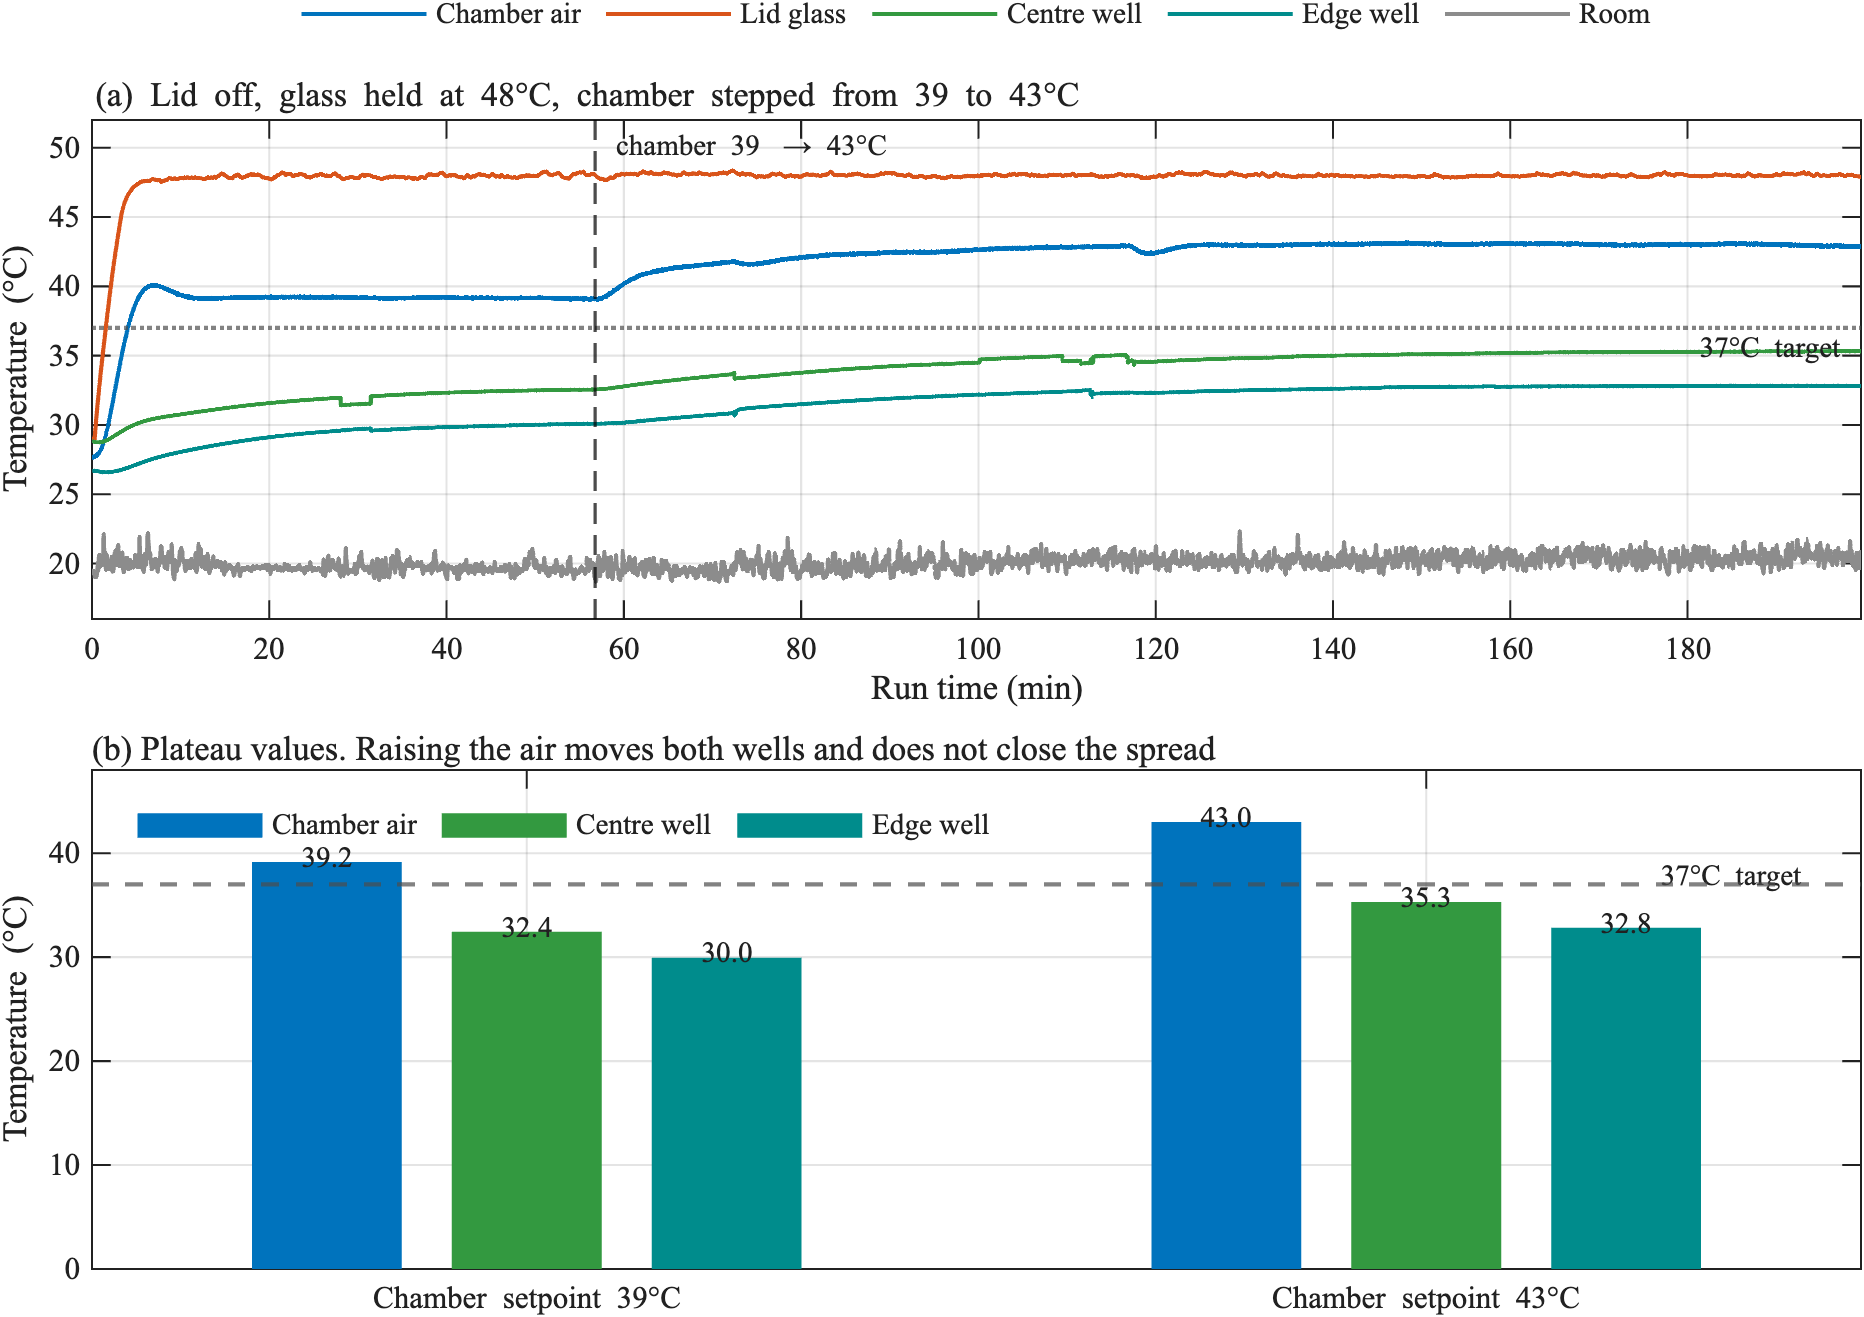
\includegraphics[width=0.66\textwidth]{figs/ch7/fig_C2_setpoint_sweep.png}
    \caption[Setpoint sweep with two wells]{\textbf{Raising the air temperature with the plate lid off.} (a) The whole run, with the chamber setpoint stepped from 39 to 43\,\textdegree{}C. (b) The two plateaus. Both wells move up together and the gap between them does not close.}
    \label{fig:C2-sweep}
\end{figure}

\begin{table}[htbp]
    \centering
    \caption{Plateau averages over 20 minutes at each setpoint, run 2.}
    \label{tab:cl-test2}
    \begin{tabular}{lcc}
        \toprule
         & \textbf{Chamber 39\,\textdegree{}C} & \textbf{Chamber 43\,\textdegree{}C} \\
        \midrule
        Chamber air        & $39.154 \pm 0.043$ & $42.988 \pm 0.068$ \\
        Glass              & $47.998 \pm 0.116$ & $48.019 \pm 0.064$ \\
        Centre well (E8)   & 32.435 & 35.298 \\
        Edge well (C11)    & 29.952 & 32.818 \\
        Room               & 19.65  & 20.44 \\
        Heater duty        & 24.7\,\% & 45.1\,\% \\
        Glass duty         & 67.0\,\% & 62.2\,\% \\
        Condensation margin & 8.84\,\textdegree{}C & 5.03\,\textdegree{}C \\
        \midrule
        Well to well spread & 2.484\,\textdegree{}C & 2.480\,\textdegree{}C \\
        \bottomrule
    \end{tabular}
\end{table}


\textbf{The sample result.} Table~\ref{tab:cl-test2} gives the two plateaus. The air went up 3.83\,\textdegree{}C and both wells went up 2.86\,\textdegree{}C, so the gap between centre and edge held: 2.484\,\textdegree{}C at 39\,\textdegree{}C air and 2.480\,\textdegree{}C at 43\,\textdegree{}C air. Raising the air lifts both wells and leaves the gap alone. Extrapolating from the plateau temperatures and a 20.4\,\textdegree{}C room, a 37\,\textdegree{}C centre well needs 45.7\,\textdegree{}C air, a 37\,\textdegree{}C edge well needs 50.6\,\textdegree{}C, and at 45.7\,\textdegree{}C air the edge well sits at 34.3\,\textdegree{}C. No air temperature puts both wells at 37\,\textdegree{}C. The cost is also high: the condensation margin drops from 8.84 to 5.03\,\textdegree{}C for less than 4\,\textdegree{}C of air, and the open wells evaporate faster. Raising the air was tested and rejected.

\textbf{The sample is also slow.} The wells reached 63.2\,\% of the step in 2105\,s for E8 and 1831\,s for C11, about half an hour, against 699\,s for the air. The loop measures the air, which settles roughly half an hour before the sample does.

\textbf{Two control results.} Heater duty rose from 24.7 to 45.1\,\% for a 3.83\,\textdegree{}C rise in air, so one percent of duty buys 0.188\,\textdegree{}C up at 43\,\textdegree{}C. Near 37\,\textdegree{}C the same figure was 0.327, which is the value the controller was tuned on. The chamber loses more heat the further it sits above the room, so a percent of duty buys about 40\,\% less at the top of the range, and the loop runs slower than designed: 699\,s against a 300\,s target. The wall heaters also heat the glass, so pushing the chamber up by 3.8\,\textdegree{}C sent extra heat into the glass. The glass loop cut its own duty from 67.0 to 62.2\,\% to compensate and held $48.00 \pm 0.10$\,\textdegree{}C across the whole run, never dropping below 47.67\,\textdegree{}C. The disturbance landed on the glass duty and left the glass temperature alone, which is what the loop separation was for.

\textbf{The warm-up overshoot.} The warm-up overshot by 1.08\,\textdegree{}C, where run 1 did not overshoot at all. The setpoints here are higher, so both loops ran at 100\,\% duty from $t = 16$\,s, the heater for 78\,s and the glass for 174\,s. Neither loop saturated in run 1, and that is the difference. While the glass loop sits at 100\,\% it cannot take back the heat the wall heaters put into the glass, so the chamber sees the full gain of 51 and acts 1.6 times harder than it was tuned for (Section~\ref{sec:sysid-gains}). The integrator also starts too high. It is set at start-up from the room temperature so the heater begins near the duty the setpoint needs, and for these setpoints that starting value works out above 100\,\%. The loop then leaves saturation with more integral action than it needs. Starting the integrator no higher than the output limit should fix it.

%*********************************************************************
\section{Heating from Below}
\label{sec:cl-test3}
%*********************************************************************

Run 2 showed the sample temperature can be reached from above, but only by running the air near 46\,\textdegree{}C, and only for one well at a time. All the heat then comes in from the top, so the liquid at the top of a well sits well above the cells on the floor. Heating from below adds a second path, so the sample is warmed from both sides and the gradient through it should be smaller. The third run tests that. The chamber was held at 39\,\textdegree{}C and the glass at 48\,\textdegree{}C, the same setpoints as run 2, with a second ITO-coated pane added under the plate and driven open loop at a fixed duty. Figure~\ref{fig:C3-base}a and b show the run.

The pane sits under the plate and so sits in the optical path of an inverted microscope. Whether it can stay there is not established here, and a heated metal frame holding the plate would give the same bottom heating with the light path clear. This run tests the principle, not a final design.

\begin{figure}[htbp]
    \centering
    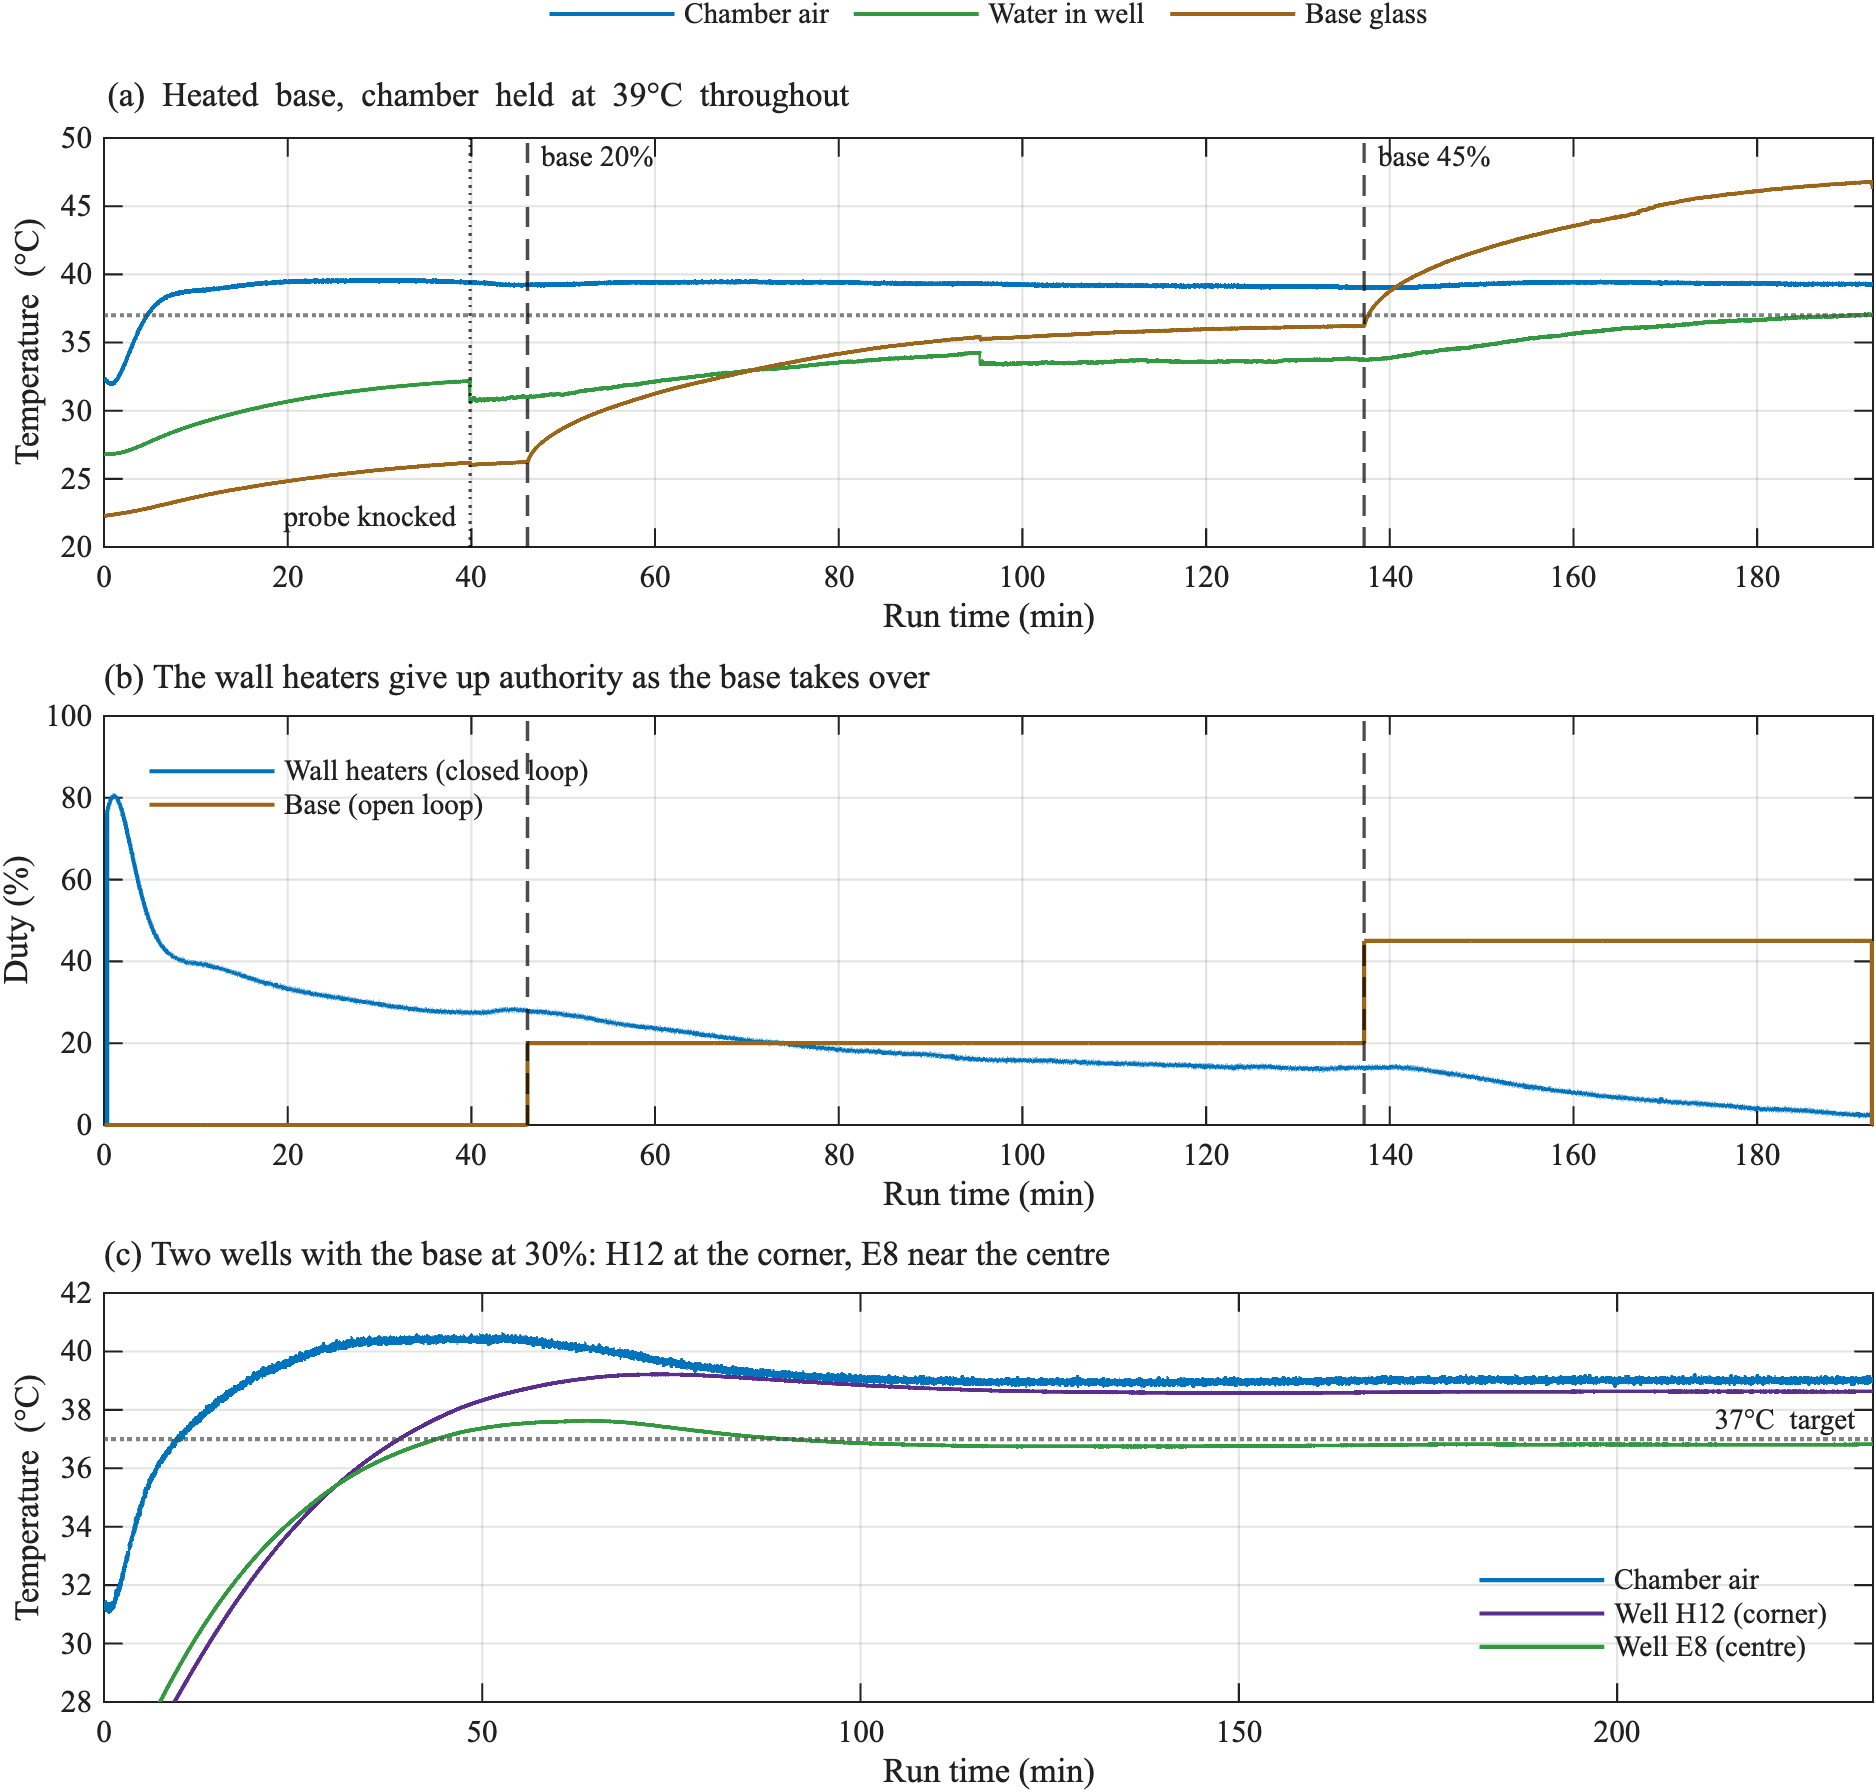
\includegraphics[width=0.66\textwidth]{figs/ch7/fig_C3_heated_base.png}
    \caption[Heated base and plate evenness]{\textbf{Heating the plate from below.} (a) Run 3, with the chamber loop holding 39\,\textdegree{}C while the base duty is raised in two steps. (b) The duties from the same run: the closed loop wall heaters back off as the open loop base takes over. (c) Run 4, two wells on opposite parts of the plate with the base at 30\,\%.}
    \label{fig:C3-base}
\end{figure}

\begin{table}[h]
    \centering
    \caption{Run 3 plateaus, with the chamber loop holding 39\,\textdegree{}C throughout.}
    \label{tab:cl-test3}
    \small
    \begin{tabular}{lcccc}
        \toprule
        \textbf{Base duty} & \textbf{Chamber air} & \textbf{Well} & \textbf{Base glass} & \textbf{Wall heater duty} \\
        \midrule
        0\,\%  & 39.27 & 30.89 & 26.15 & 27.9\,\% \\
        20\,\% & 39.16 & 33.60 & 35.84 & 14.7\,\% \\
        45\,\% & 39.31 & 36.67 & 46.10 & 4.0\,\% \\
        \bottomrule
    \end{tabular}
\end{table}

The well rose from 30.9 to 36.7\,\textdegree{}C, 5.8\,\textdegree{}C, while the air stayed at 39.3\,\textdegree{}C. Run 2 needed the air at 45.7\,\textdegree{}C to reach the same place and still left the edge well 3\,\textdegree{}C short. Heating from below therefore does what raising the air cannot, and it does it while the condensation margin stays near 8.6\,\textdegree{}C instead of falling.

The duties in Figure~\ref{fig:C3-base}b are the other half of the result. The wall heaters fell from 27.9 to 4.0\,\% as the base came up, so at 45\,\% base duty the base supplies nearly all the heat and the chamber loop sits almost at zero duty. From there it can only take out another 4 points, so it can no longer hold the air down if anything pushes it up. That is a control consequence worth stating: an open loop base is a disturbance to the closed loop above it, and with the base much hotter than the air the chamber loop ends up trimming rather than heating. A future version would have to close a loop around the base as well, which is also what would let it hold 37\,\textdegree{}C at the sample directly rather than through the air.

\textbf{Measurement caveat.} The well probe was knocked twice during this run, at $t = 2392$\,s when the bench was bumped and again at about $t = 5740$\,s, dropping the reading by 1.2\,\textdegree{}C and then 0.6\,\textdegree{}C with every other channel unchanged. The 0\,\% plateau in Table~\ref{tab:cl-test3} is taken after the first disturbance, so the 5.8\,\textdegree{}C total carries about 0.6\,\textdegree{}C of uncertainty from the second. The two undisturbed segments give 2.7\,\textdegree{}C from 0 to 20\,\% and 3.1\,\textdegree{}C from 20 to 45\,\%, which adds to the same 5.8\,\textdegree{}C without using any data from around the knocks.

%*********************************************************************
\section{Evenness Across the Plate}
\label{sec:cl-test4}
%*********************************************************************

Run 2 found a 2.5\,\textdegree{}C spread between E8 near the centre and C11, one column in from the edge. The last run repeats that measurement with the heated base in place and moves the outer probe to H12, the corner well and the most exposed position on the plate. The base ran open loop and the chamber loop held 39\,\textdegree{}C. The base was started at 45\,\% and reduced to 30\,\% once the plate was clearly overshooting. Figure~\ref{fig:C3-base}c shows the run, which was the cleanest of the four: over the last two hours the two well channels held to within 0.005\,\textdegree{}C.

\begin{table}[htbp]
    \centering
    \caption{Run 4, averaged over the last 20 minutes with the base at 30\,\%.}
    \label{tab:cl-test4}
    \small
    \begin{tabular}{lccccc}
        \toprule
         & \textbf{Chamber} & \textbf{Glass} & \textbf{Well E8} & \textbf{Well H12} & \textbf{Wall heater duty} \\
        \midrule
        Mean    & 39.006 & 47.949 & 36.811 & 38.625 & 13.0\,\% \\
        Std dev & 0.040  & 0.114  & 0.003  & 0.005  & 0.33 \\
        \bottomrule
    \end{tabular}
\end{table}

Table~\ref{tab:cl-test4} gives the final 20 minutes. Both wells are now close to target, the centre at 36.81\,\textdegree{}C and the corner at 38.63\,\textdegree{}C, against 32.4 and 30.0\,\textdegree{}C without base heating in run 2. The corner figure is the stronger of the two, since H12 sits further out than the C11 well it is being compared against. The centre well is 0.19\,\textdegree{}C from target, the first well temperature in specification in the project.

The gradient has also reversed. Without base heating the centre well was 2.5\,\textdegree{}C warmer than the outer well, because the plate rim loses heat to the housing. With base heating the corner is 1.81\,\textdegree{}C warmer than the centre, because the base pane is driven through copper busbars along two of its edges, so the rim is now where heat enters. The spread has fallen from 2.5 to 1.8\,\textdegree{}C and the sign follows whichever rim path is stronger. The plate edge is the hard part either way, and the base layout sets it, not the air.

The spread is still larger than R2 allows, and no single open loop base duty removes it. At 30\,\% the centre is 0.2\,\textdegree{}C low and the corner 1.6\,\textdegree{}C high, and lowering the duty to bring the corner down takes the centre further below target. Putting the base under closed loop control would set the average well temperature but would leave the two wells apart, since the busbars feed heat in along two edges only. An even plate temperature needs the busbars moved to opposite long edges with a more uniform sheet resistance, or the base split into two zones. Both are taken up in Chapter~\ref{ch:furtherwork}.

%*********************************************************************
\section{Summary}
\label{sec:cl-summary}
%*********************************************************************

The chamber held $37.028 \pm 0.038$\,\textdegree{}C over 80 minutes. That spread is the same size as the converter's smallest step of 0.034\,\textdegree{}C, so the loop is as steady as the instrument can show, and its full 0.24\,\textdegree{}C span uses less than half of the $\pm$0.3\,\textdegree{}C of R1. Opening the chamber cost 0.39\,\textdegree{}C and 1.6 minutes to recover, on 3.4 extra percentage points of duty, and about 1\,\textdegree{}C of room drift passed through with no visible effect. The glass held its own setpoint through a 3.8\,\textdegree{}C move in the chamber and settled 2.3 times faster, which is what keeps the two loops from fighting. The parameters identified at 25 to 30\,\textdegree{}C in Chapter~\ref{ch:thermalID} therefore hold at 37\,\textdegree{}C.

R2 is not met. Holding the air at 37\,\textdegree{}C leaves the sample at 34.4\,\textdegree{}C, and run 2 showed that cannot be fixed from above: both wells move with the air at the same rate, so raising the setpoint lifts both and leaves the 2.5\,\textdegree{}C spread between them, and no air temperature puts both at 37\,\textdegree{}C. Heating the plate from below does work, lifting the well from 30.9 to 36.7\,\textdegree{}C with the air unchanged. Run 4 put a well within 0.2\,\textdegree{}C of target for the first time, with the spread down to 1.8\,\textdegree{}C and its sign reversed.

Three things need work. The heated base ran open loop, and at the duties needed it leaves the chamber loop almost nothing to act with, so it needs its own controller. The remaining spread is set by where the base busbars sit and not by the control. And one percent of duty buys only about 60\,\% as much air temperature at 43\,\textdegree{}C as at 37\,\textdegree{}C, so the loops are slower away from the point they were tuned at.

%*********************************************************************
% End of Closed Loop Thermal Performance
%*********************************************************************